%!TEX program = xelatex
\documentclass{ctexart}

\usepackage{seustyle}
\usepackage{amsmath}
\usepackage{bm}
\usepackage{tikz}
\usetikzlibrary{calc}
\usetikzlibrary{external}
\tikzexternalize
\tikzsetexternalprefix{figures/}

\title{输电塔表面所受龙卷风风压转化为塔结构梁单元节点集中力的算法}
\author{王勇}
\date{}

\begin{document}

\graphicspath{{figures/}}

\maketitle

% \begin{abstract}
% 	xxx
% \end{abstract}

\section{引言}
% 现在的技术路线及存在的问题;
% 输电塔选择梁单元建模可以减少计算量;
% 采用梁单元引出新的问题:如何将输电塔表面受到的龙卷风风压转化为梁单元荷载?
在Workbench平台下进行龙卷风风场中输电塔结构的单向流固耦合分析的思路为:
建立考虑输电塔刚性模型的龙卷风风场,通过fluent计算得到刚性输电塔表面的风压分布;
将CFD计算的风压映射到ANSYS Mechanical的表面效应单元SURF154上,进而加载到输电塔壳单元上;
在ANSYS Mechanical中进行有限元分析。

这种方法在Workbench平台下容易实现(程序可自动将CFD风压映射到结构有限元网格)。
但这种方法要求结构必须以实体单元或壳单元离散才能实现CFD风压的映射,计算量巨大。
本文采用梁单元模拟输电塔结构,具有建模简单、有限元计算量较小等特点,但也引入了新的问题:
即CFD计算得到的风压分布如何传递到梁单元上?

\section{算法}
% 核心算法,判断CFD Pressure Points分别作用于哪个梁单元?
% 单个CFD Pressure Point风压分解为整体直角坐标系的分量。
% 某个梁单元所受全部CFD Pressure Points的风压分量的平均与该梁单元节点荷载计算。
% CFD计算得到的输电塔刚性模型表面的风压分布可导出成表\todo{Insert CFD Pressure Data Format}。
由于流场网格对刚性输电塔表面的离散,使得风压点的位置与实际的输电塔结构表面存在偏差。
因此需要设计算法实现如下功能:

\begin{figure}[!htbp]
    \centering
    \input{figures/algo.tikz}
    \caption{CFD风压点$P$与梁单元$IJ$示意图}
    \label{fig:algo}
\end{figure}

\begin{itemize}
	\item 判别每个CFD风压点作用于哪个有限元梁单元。
	\item 将单个CFD风压点的风压(垂直于该风压点作用的梁单元的表面)分解到整体坐标系中。
	\item 将单个有限元梁单元所受所有CFD风压点的压力进行合成,并分配到该单元节点上。
\end{itemize}

任意CFD风压点$P$与某个梁单元$IJ$示意图见图\ref{fig:algo},图中点$P'$为风压点$P$在梁单元轴线$IJ$上的投影。
由于本文研究的输电塔为钢管塔,即梁$IJ$的表面为柱面,设其外径为$R_{IJ}$,则$PP'$即为风压作用于梁$IJ$的方向。
首先通过如下准则判断风压点$P$是否作用于梁单元$IJ$上:
\begin{itemize}
	\item $P'$是否在线$IJ$内部?
    \item $PP'$是否近似等于单元$IJ$外径?
\end{itemize}
当同时满足这两个条件时,认为风压点$P$作用于梁单元$IJ$上,数学表达见式\eqref{eqn:cri}。
\begin{gather}\label{eqn:cri}
\bm{P'I}\cdot\bm{P'J} < 0  \nonumber \\
|PP'-R_{IJ}| < \epsilon
\end{gather}
式中点$P'$的坐标可由式\eqref{eqn:op}计算,
\begin{equation}\label{eqn:op}
\bm{OP'}=\bm{OI} - \left( \frac{\bm{PI}\cdot\bm{IJ}}{|IJ|^2} \right)\bm{IJ}
\end{equation}
风压点$P$作用于梁单元$IJ$上的风压在整体坐标系下的分量为
\begin{equation}
(p_X, p_Y, p_z) = p\frac{\bm{PP'}}{|PP'|}
\end{equation}

根据上述判别法则,对每个CFD风压点与每根梁单元进行判别,可确定每根梁单元所受的所有CFD风压点及各自的风压分量。
下面介绍将单个有限元梁单元所受所有CFD风压点的压力进行合成,并分配到该单元节点上的方法。
\begin{enumerate}
\item 计算单个有限元梁单元$IJ$受到的所有风压点处风压分量的平均$\bar{p_X},\bar{p_Y},\bar{p_Z}$;
\item 将风压根据梁表面面积转化为合力$F_X=2\pi R_{IJ} |IJ| \bar{p_X}$,$Y,Z$方向类似;
\item 将风压合力分量平分到梁单元$I$、$J$节点上。
\end{enumerate}
至此,完成了将CFD风压传递给有限元梁单元节点荷载的算法。

\newpage

\section{测试算例}
% 圆柱绕流问题。
设计如图\ref{fig:example}所示的算例测试该算法的有效性。
悬臂钢管柱外径$R=\SI{1.0}{m}$,高度$H=\SI{9}{m}$,单侧受到径向压强,分布为$p_r(y)=p_0\frac{y}{H},p_0=\SI{100}{Pa}$。
据此编程生成风压点及相应的压强值,作为本文算法的输入,输出各节点施加的集中力如图\ref{fig:force}所示。
同时输出各节点集中力的合力见图\ref{fig:force_sum}所示,与理论合力$F_X = \int_{0}^{H}\int_{\pi/2}^{3\pi/2}p_r(y)\cos(\theta+\pi)R \mathrm{d} \theta \mathrm{d} y = p_0 RH=\SI{900}{Pa}$误差很小。
\begin{figure}[!htbp]
    \centering
    \input{figures/example.tikz}
    \caption{测试算例示意图}
    \label{fig:example}
\end{figure}

\begin{figure}[!htbp]
    \centering
    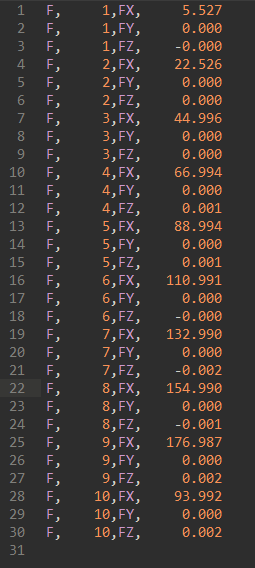
\includegraphics{figures/force.png}
    \caption{输出梁单元节点集中力的APDL程序}
    \label{fig:force}
\end{figure}

\begin{figure}[!htbp]
    \centering
    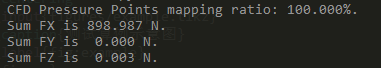
\includegraphics{figures/force_sum.png}
    \caption{程序计算的合力}
    \label{fig:force_sum}
\end{figure}

% \bibliographystyle{seuthesix}
% \bibliography{main}

\end{document}